%%
% TUM Corporate Design LaTeX Templates
% Based on the templates from https://www.tum.de/cd
%
% Feel free to join development on
% https://gitlab.lrz.de/tum-templates/templates
% and/or to create an issue in case of trouble.
%
% tum-presentation class for scientific talks, thesis presentations, ...
%
%%

%\documentclass[4to3]{tum-presentation}
%\documentclass[navsym]{tum-presentation}
%\documentclass[nothreeliner]{tum-presentation}
%\documentclass[handout,4on1]{tum-presentation}
%\documentclass[handout,2on1]{tum-presentation}
%\documentclass[handout]{tum-presentation}
\documentclass{tum-presentation}
\usepackage[font=small,labelfont=bf]{caption}
\addbibresource{literature.bib}

\title[Shortened Title]{Clustering-Based Sentiment Analysis for Media Agenda Setting}
\subtitle{Opinion Lab Group 2.3, presentation 4}
\author{Wing Sheung Leung, Qiaoxi Liu}
%\institute[]{\inst{1} Department of Electrical and Computer Engineering,
%  Technical University of Munich (TUM)\\
%  \inst{2} Department of Informatics, Technical University of Munich (TUM)}
%\date{International Conference on Mostly Scientific Topics}

\footline{\insertshortauthor~| \inserttitle}


\begin{document}


\begin{frame}[noframenumbering]
  \titlepage
\end{frame}


\begin{frame}
  \frametitle{Milestones}
  \vspace{2cm}
 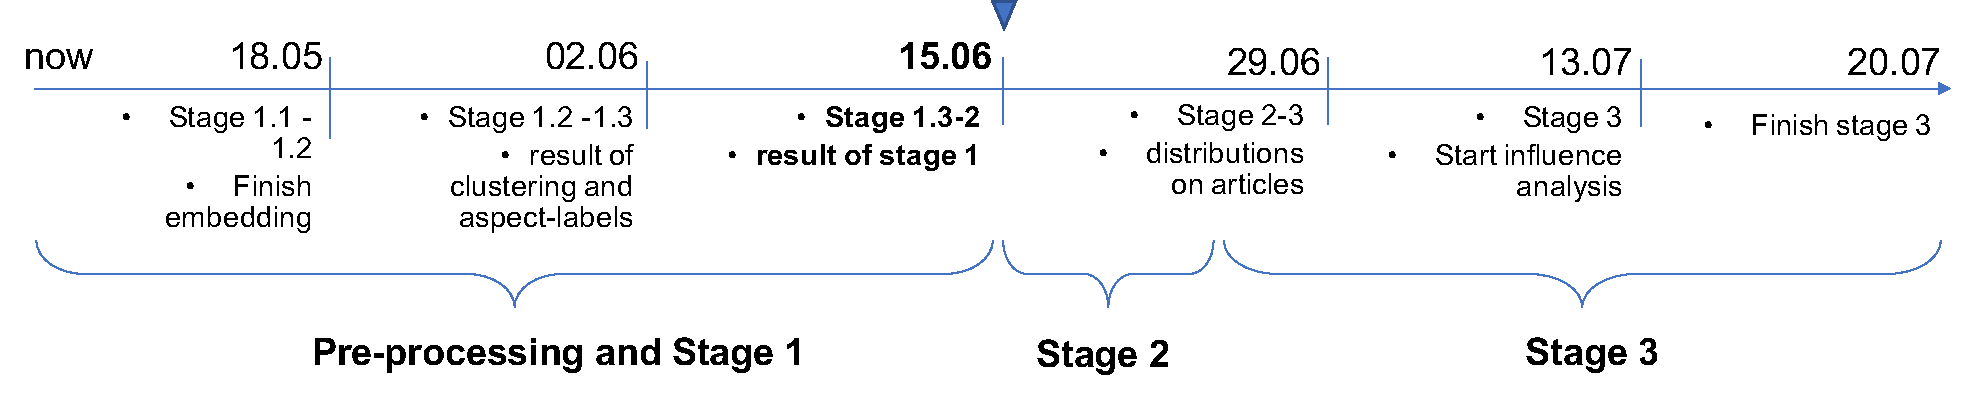
\includegraphics[width = \textwidth]{figures/timeline.pdf}
\end{frame}


\begin{frame}[t]
  \frametitle{Overview}
  \tableofcontents[sectionstyle=show,subsectionstyle=show,subsubsectionstyle=shaded]
\end{frame}


\section{Stage 1: Generate sentence embeddings with our corpus}
\subsection[shaded]{1.1 Embeddings}
\subsubsection{XLING sentence-level embeddings}
\subsubsection{Indexing sentences}
\subsection{1.2 Kmeans and determining optimal k}
\subsubsection{sklearn.cluster.MiniBatchKMeans}
\subsubsection{sklearn.cluster.KMeans}


\subsubsection{Elbow Method, AIC and BIC}
\begin{frame}
  \frametitle{Selecting global minimum in AIC as desired k}
  \framesubtitle{k = 16}
  \begin{center}
    \begin{figure}[t]
      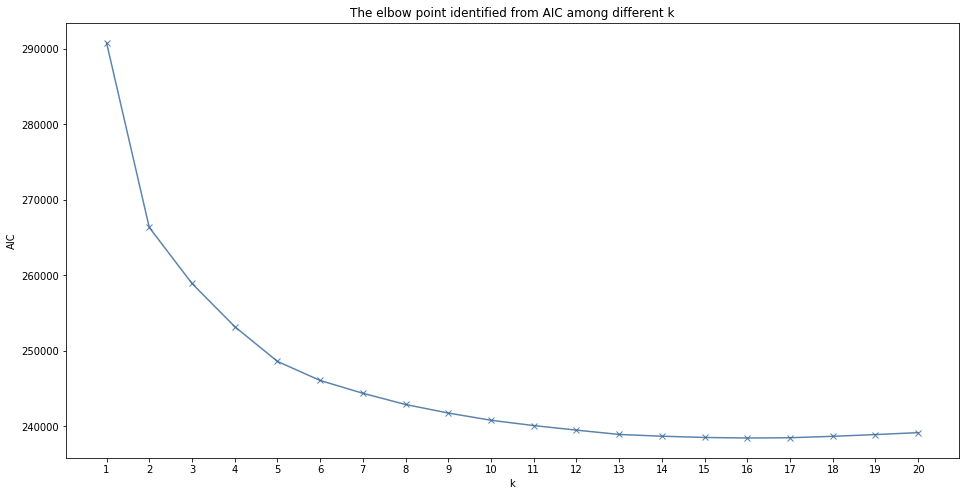
\includegraphics[width=0.6\textwidth]{images/kmean-AIC.png}
      \caption{Steeper slopes are found from k = 1 to 5, and the changes becomes gentler from k = 5 to 14. Then, it is almost flat from k = 14 to 16. It reaches \textbf{the lowest point when k = 16} and starts going up very slowly.}
    \end{figure}
  \end{center}
\end{frame}


\subsubsection{Generate topwords list with naive method and clarity scoring} %ClarityscoreGenerator vs. word frequency
\begin{frame}
  \frametitle{Word cloud generated by naive method (Recap) I}
  \framesubtitle{Naive method: sorting 1-gram words by their own frequencies within a cluster with NLTK and customized stopwords and stemming}
  \begin{center}
    \begin{figure}[t]
      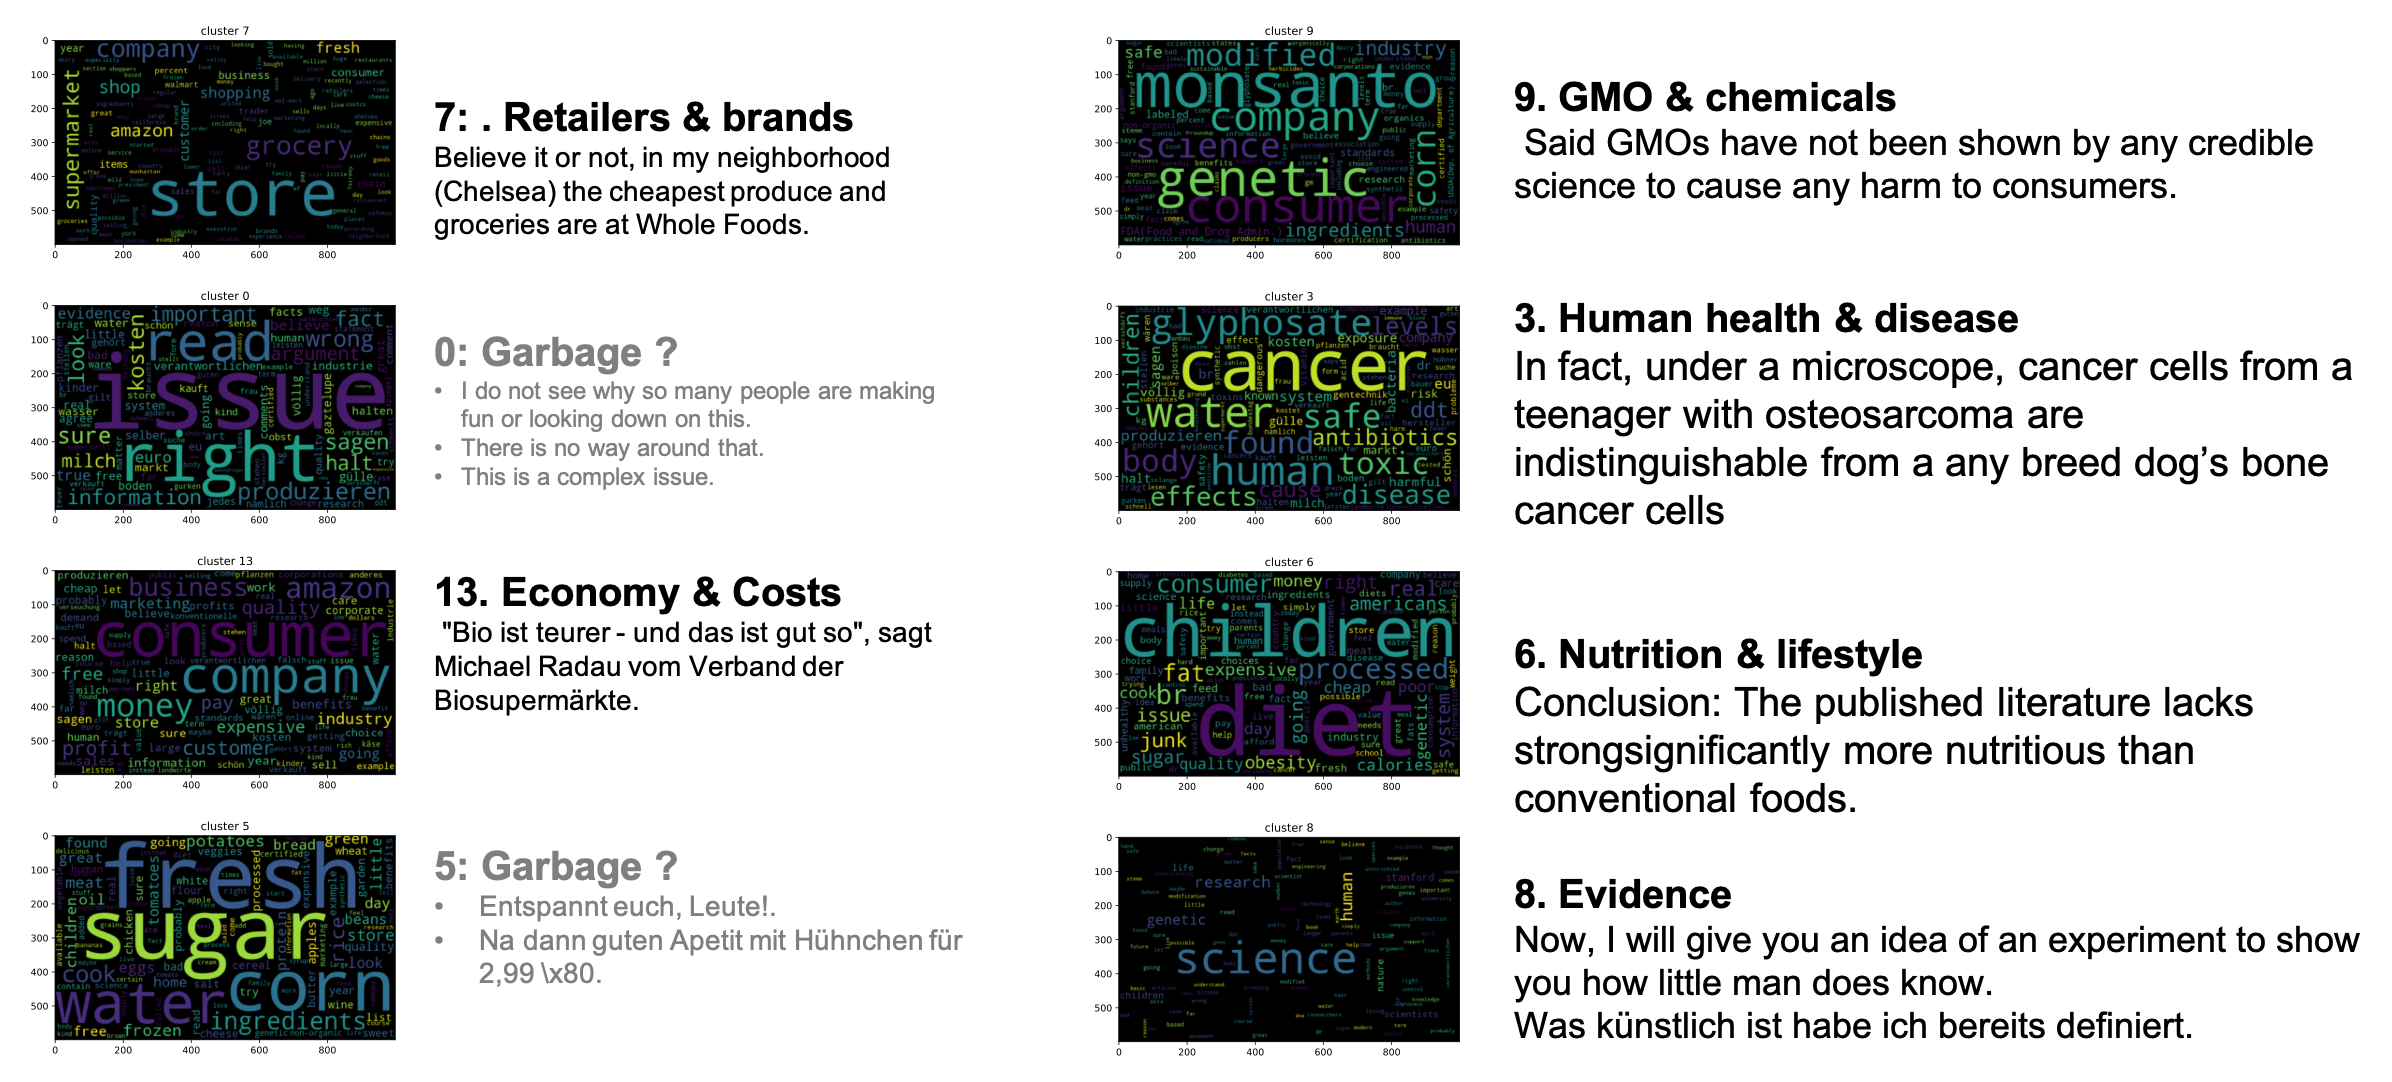
\includegraphics[width=0.8\textwidth]{figures/example16_1.png}
      \caption{First part of word cloud generated by naive method for 8 clusters with sample sentences}
    \end{figure}
  \end{center}
\end{frame}

\begin{frame}
  \frametitle{Word cloud generated by naive method (Recap) II}
  \begin{center}
    \begin{figure}[t]
      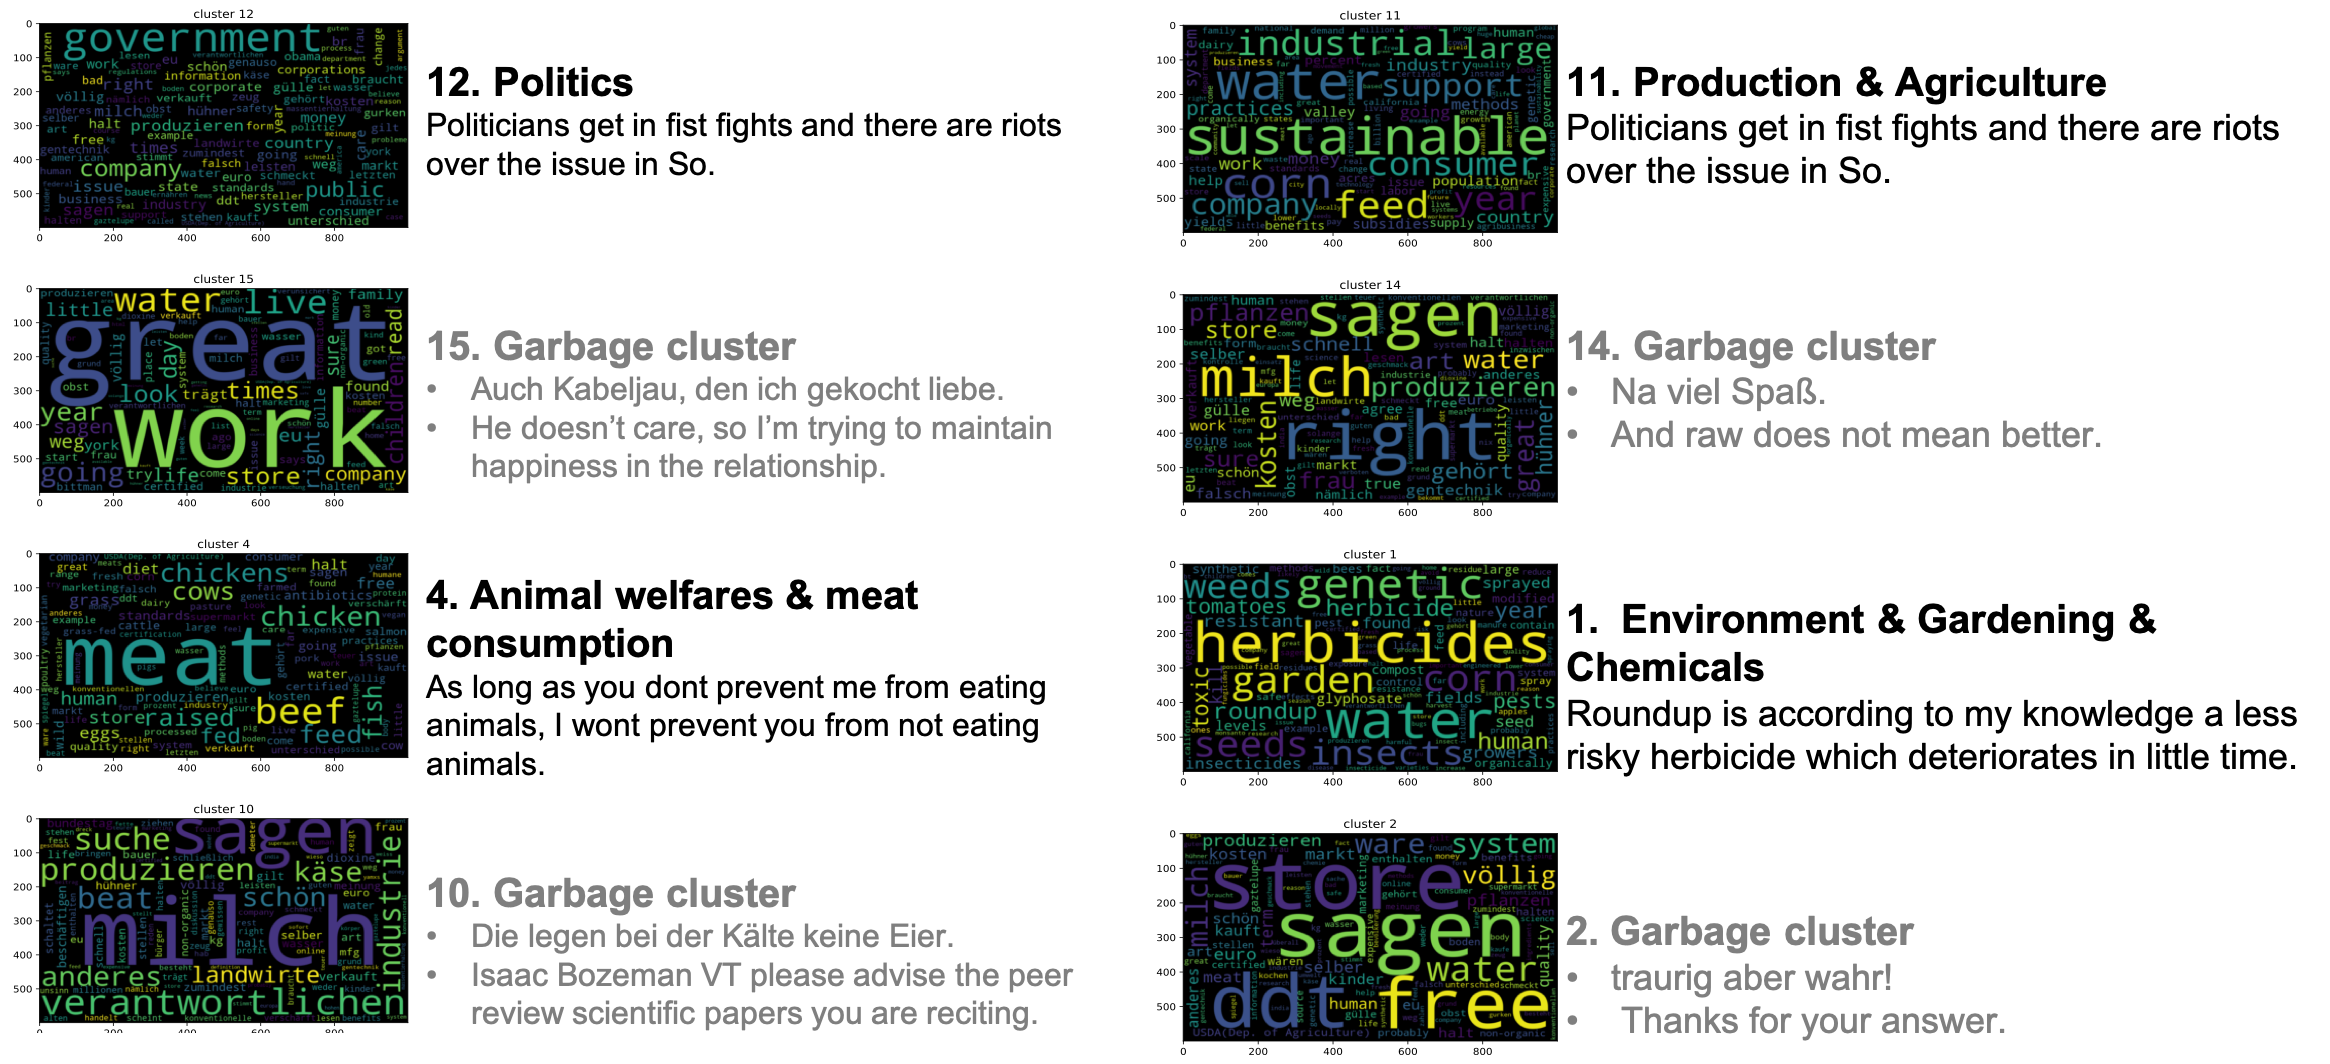
\includegraphics[width=0.8\textwidth]{figures/example16_2.png}
      \caption{Second part of word cloud generated by naive method for 8 clusters with sample sentences}
    \end{figure}
  \end{center}
\end{frame}

\begin{frame}
  \frametitle{Word cloud generated with clarity scoring I}
  \framesubtitle{Clarity scoring: measuring how much more likely to observe a word w in topic k}
  The more positive the clarity score, the more important the word to be existed in topic k \\
  \begin{center}
    \begin{figure}[t]
      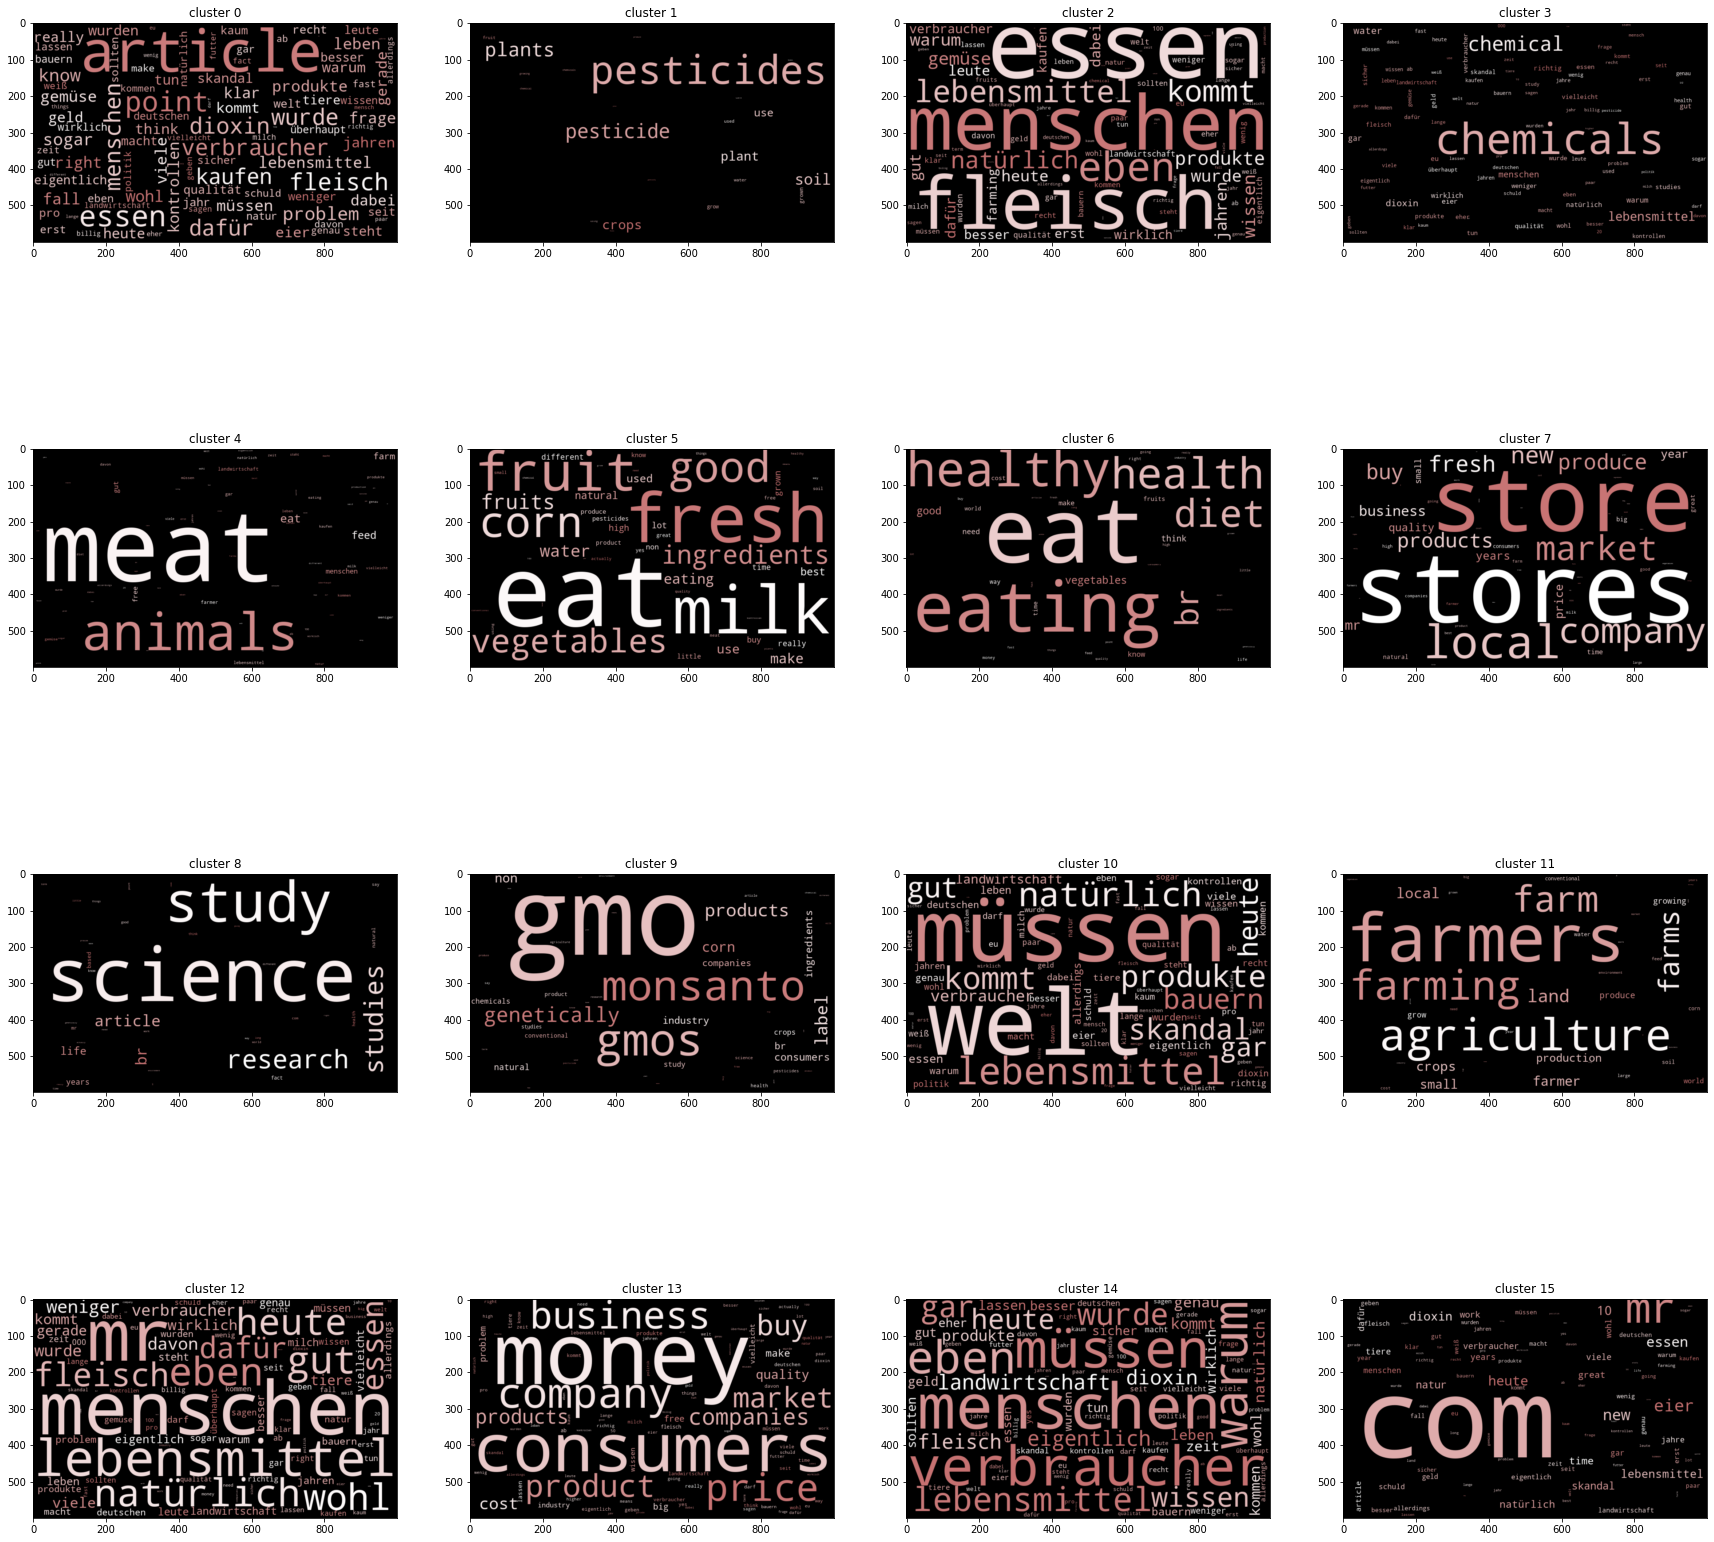
\includegraphics[width=0.36\textwidth]{images/nltk_sklearn_wordcloud.png}
      \caption{Word cloud generated with clarity scores with stopwords defined by \emph{NLTK, sklearn and some terms existing in all clusters}}
    \end{figure}
  \end{center}
\end{frame}

\begin{frame}
  \frametitle{Word cloud generated with clarity scoring II}
  \framesubtitle{With other stopwords}
  Mentioned in \cite{stopwords} \emph{"On stopwords, filtering and data sparsity for sentiment analysis of Twitter"}, based on Zipf's law, stopwords can be selected among
  \begin{enumerate}
  \item most frequent words (TF-High)
  \item words occured once, i.e. singleton words (TF1)
  \item words with low inverse document frequency (IDF)
  \end{enumerate}
  \begin{center}
    \begin{figure}[t]
      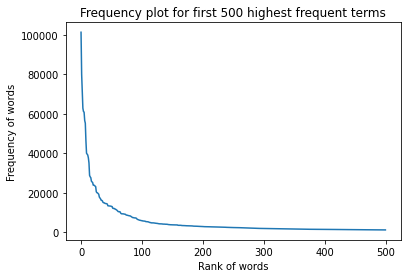
\includegraphics[width=0.29\textwidth]{images/tf-plot.png}
      \caption{The term frequency plot fits Zipf's law, which states the most frequent word will occur approximately twice as often as the second most frequent word, three times as often as the third most frequent word, etc.}
    \end{figure}
  \end{center}
\end{frame}

\begin{frame}
  \frametitle{Word cloud generated with clarity scoring III}
  Stopwords: the first 430 most frequent terms (TF-High) except 73 potential topic related terms (e.g. pesticides, farmer and GMO)
  \begin{center}
    \begin{figure}[t]
      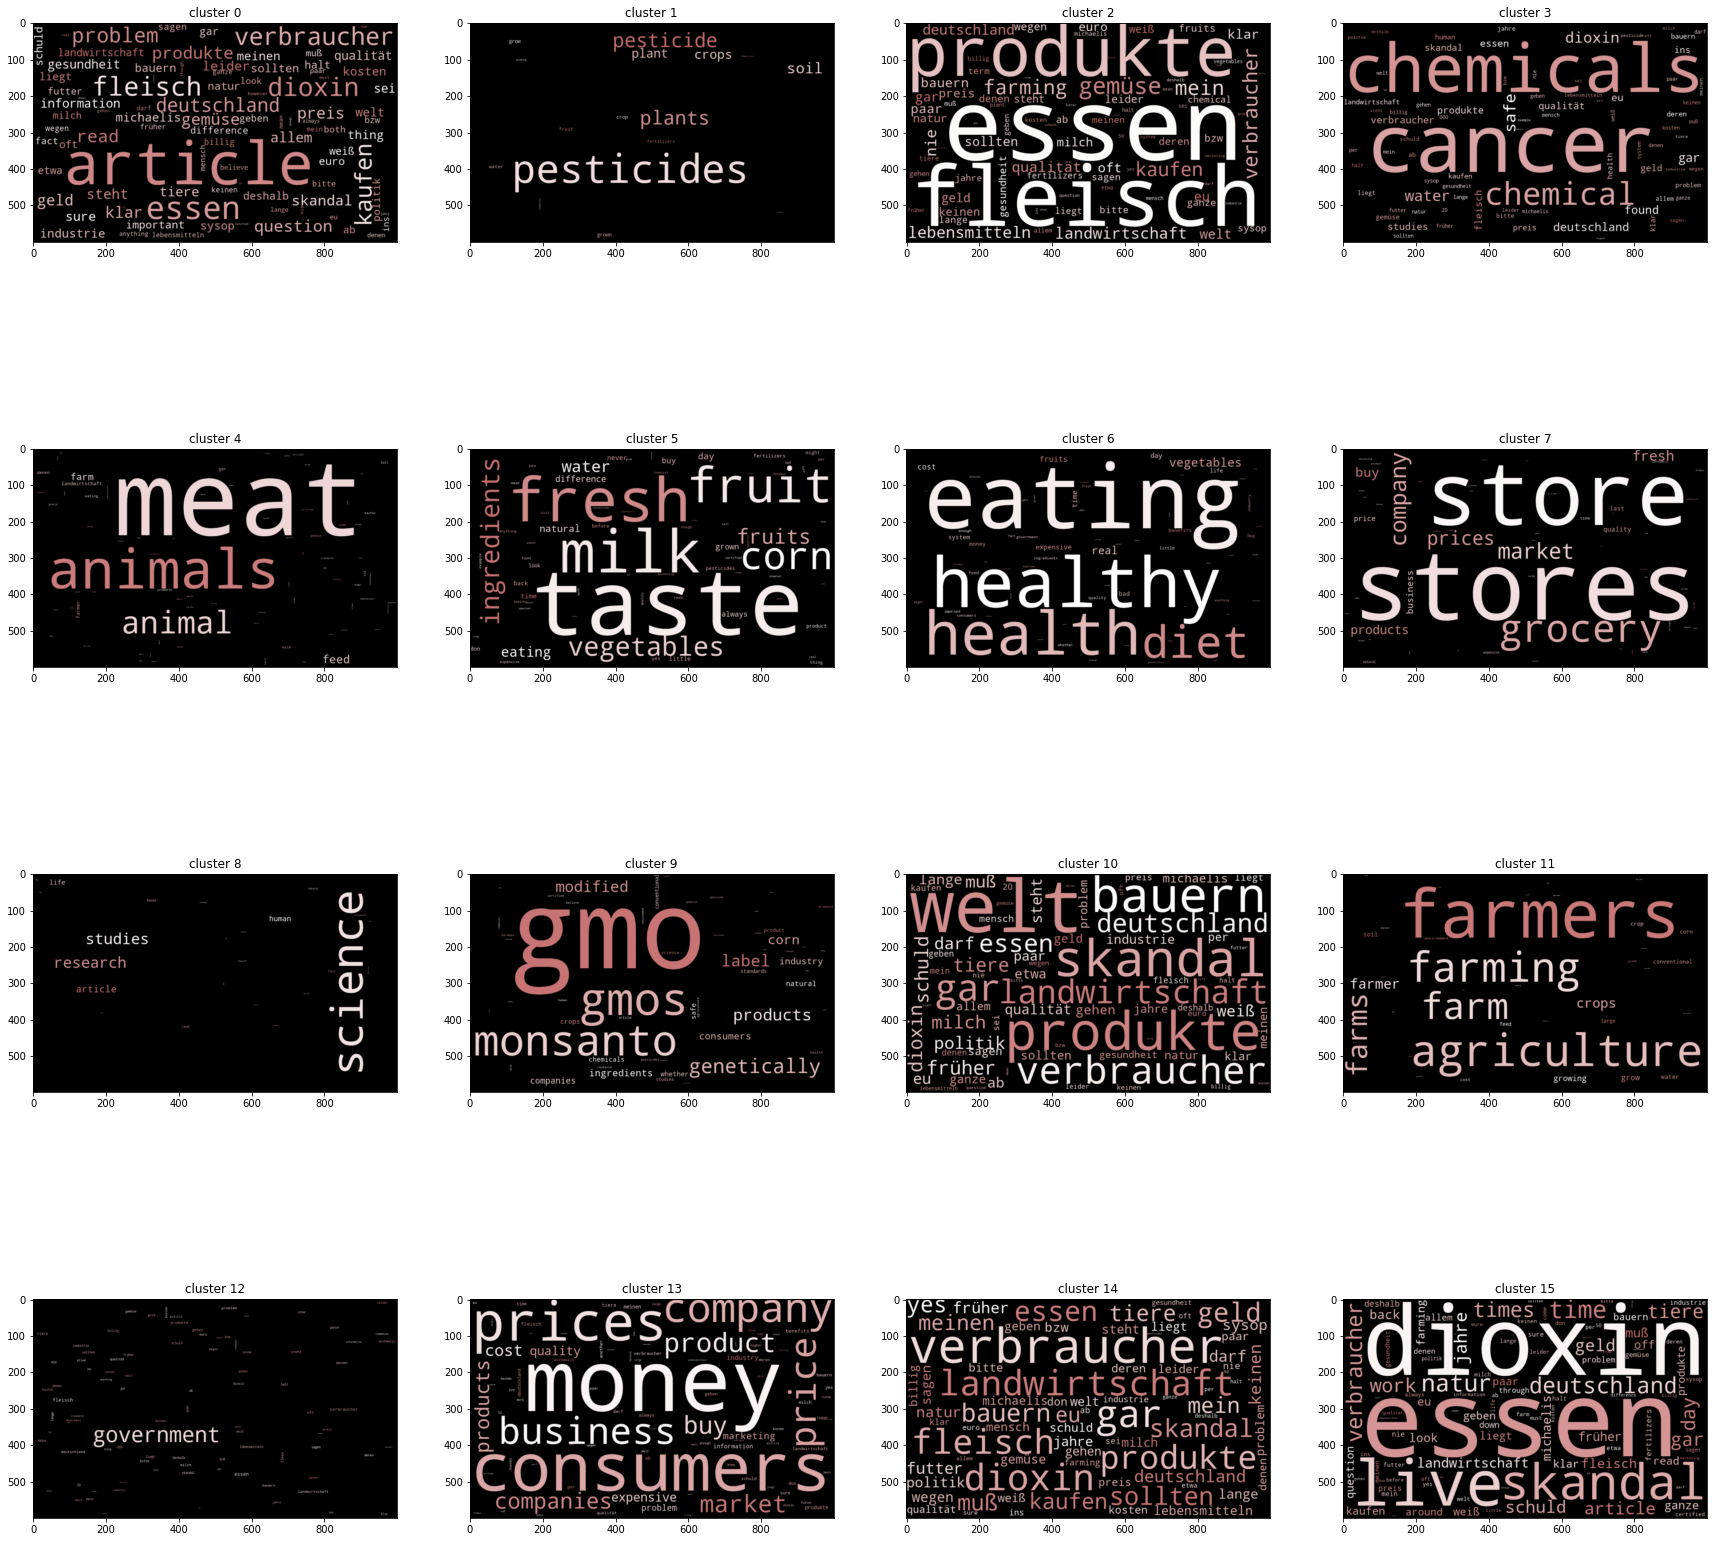
\includegraphics[width=0.36\textwidth]{images/tfhigh_wordcloud.png}
      \caption{Word cloud generated with clarity scores with \emph{TF-High} stopwords}
    \end{figure}
  \end{center}
\end{frame}

\begin{frame}
  \frametitle{Word cloud generated with clarity scoring IV}
  Stopwords: singleton words (TF1)
  \begin{center}
    \begin{figure}[t]
      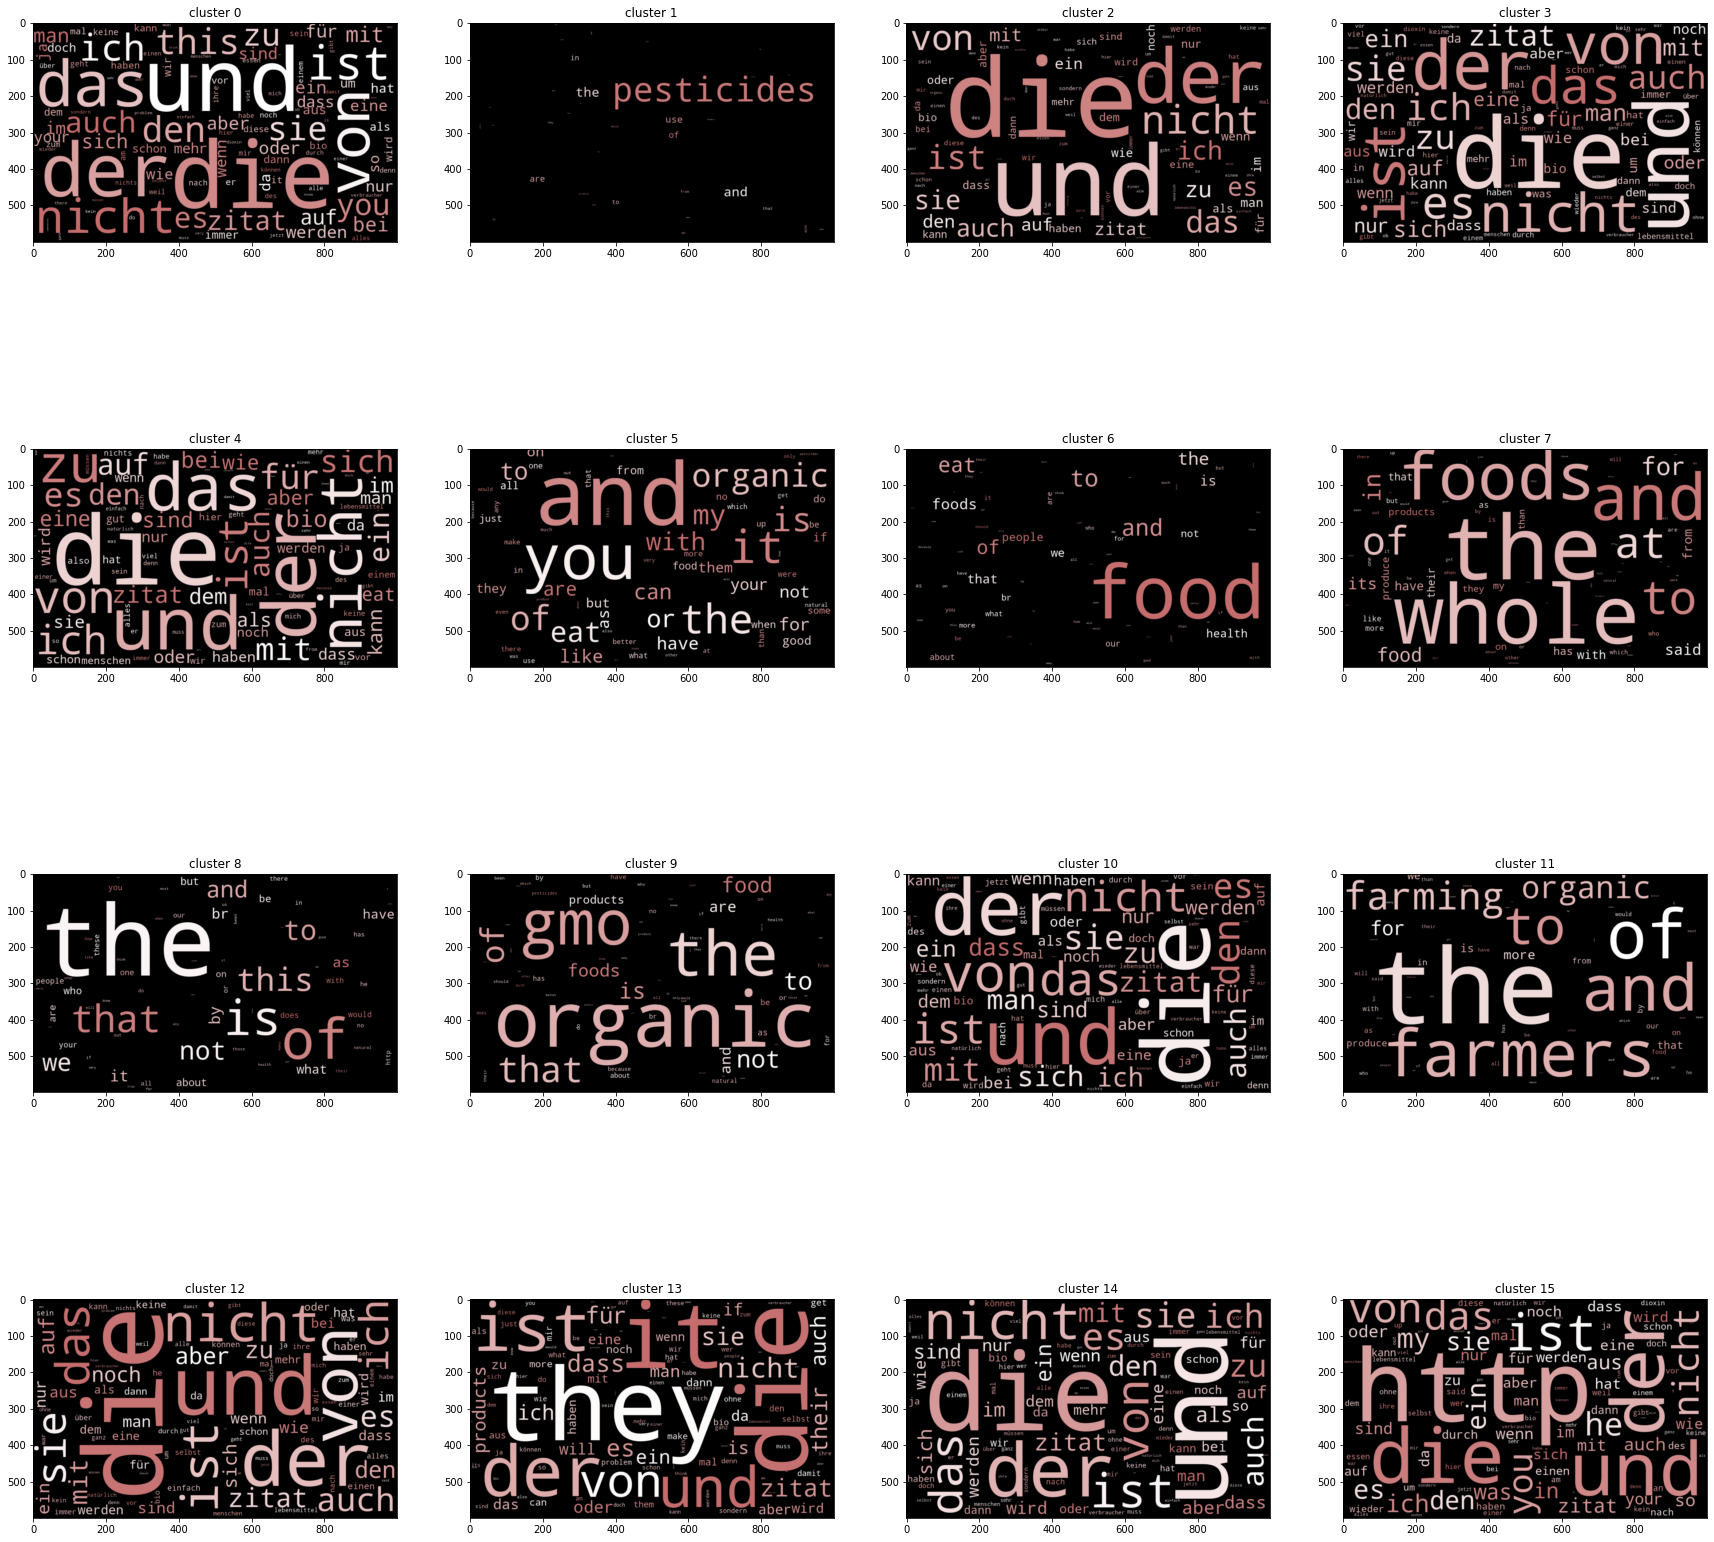
\includegraphics[width=0.36\textwidth]{images/tf1_wordcloud.png}
      \caption{Word cloud generated with clarity scores with \emph{TF1} stopwords}
    \end{figure}
  \end{center}
\end{frame}

\begin{frame}
  \frametitle{Topwords and garbage clusters}
  \begin{table}[]
    \begin{tabular}{c|l|l}
    \hline
    Cluster & Topic name & Top words sorted by clarity scores\\ \hline
    0       & Garbage                & -                                                                       \\
    1       & Planting and gardening & pesticide, plant, soil, crop, grow, fruits, water, fertilizer           \\
    2       & Garbage                & -                                                                       \\
    3       & Chemicals and cancer   & cancer, chemical, safe, water, dioxin, gar, verbraucher                 \\
    4       & Meat and animals       & meat, animal, feed, farm, landwirtschaft, farmer, gar                   \\
    5       & Taste and food         & taste, fresh, milk, fruit, corn, vegetables, ingredients                \\
    6       & Health and diet        & eating, health, diet, vegetables, real, fruits, life                    \\
    7       & Retail                 & store, grocery, company, market, price, fresh, buy                      \\
    8       & Scientific research    & science, studies, research, article, human, life, read                  \\
    9       & GMO                    & gmo, monsanto, genetically, label, products, modified, corn             \\
    10      & Skandals               & welt, produkte, skandal, dioxin, schuld, milch, politik                 \\
    11      & Agriculture            & farmer, agriculture, crop, grow, soil, water, conventional              \\
    12      & Polices                & government, fleisch, verbraucher, tiere, landwirtschaft, times, problem \\
    13      & Economy                & money, consumers, price, company, business, product, marketing          \\
    14      & Garbage                & -                                                                       \\
    15      & Garbage                & -                                                                       \\ \hline
    \end{tabular}
  \end{table}
\end{frame}


\subsection{1.3 Generation of (cluster, sentiment) tuples to each sample sentence}
\subsubsection{Extracting topics from clustering results}
\subsubsection{Assigning sentiment by pre-trained model}
\begin{frame}
  \frametitle{Recap our journey}
 
  \begin{figure}[t]
    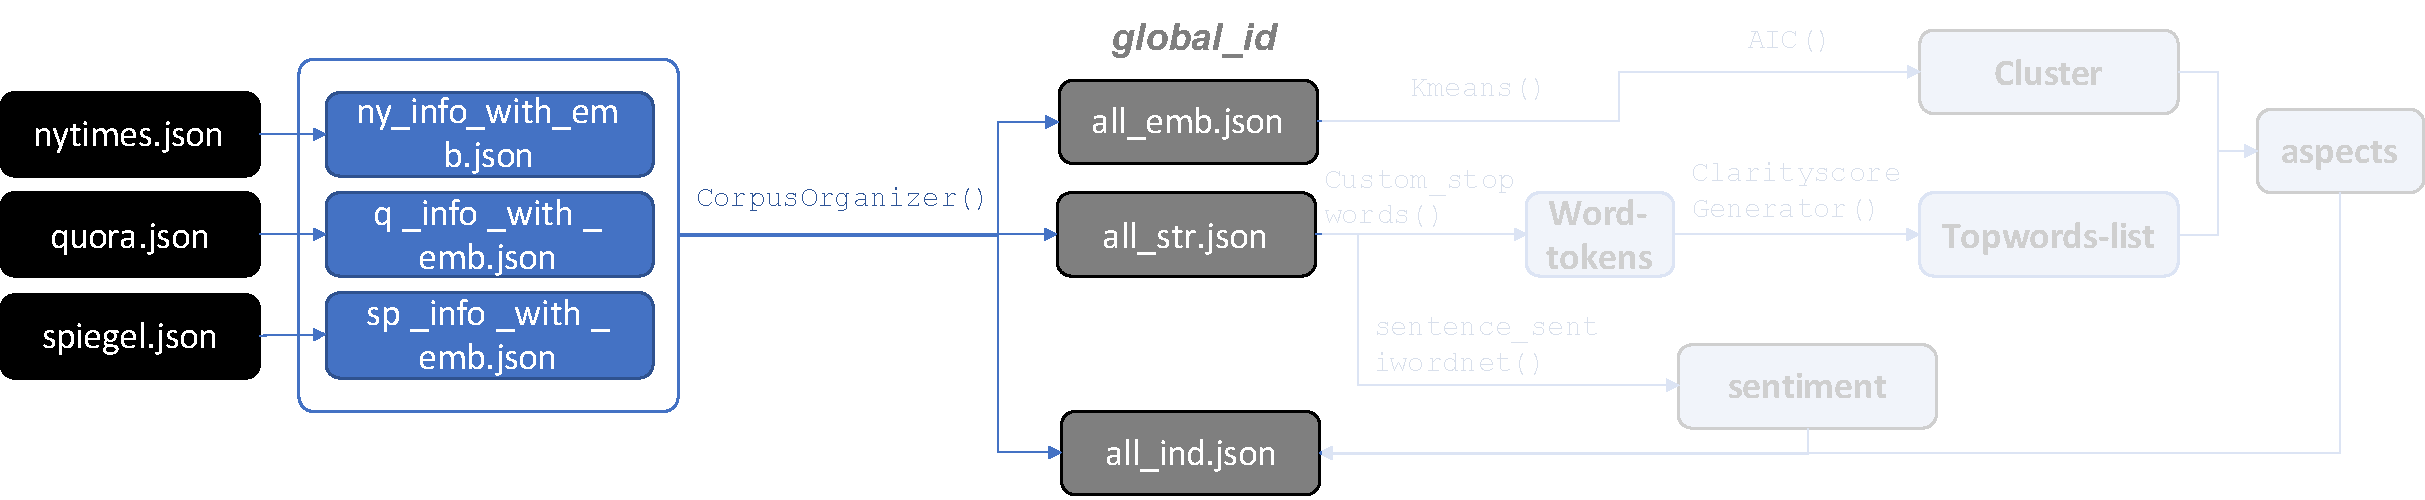
\includegraphics[width = \textwidth]{figures/journey0.pdf}
    \end{figure}

Example sentence: \textit{"Like most grocery chains, Whole Foods does not release sales data on individual stores."}
\\[2ex]
\begin{tabular}{|r|l|r|r|}
      global\_id & corpus\_name &  doc\_id &  com\_id  \\
     
      30120 &     nytimes &     191 &     NaN  \\
      \end{tabular}
\end{frame}

\begin{frame}
  \frametitle{We are now here!}
    
  \begin{figure}[t]
    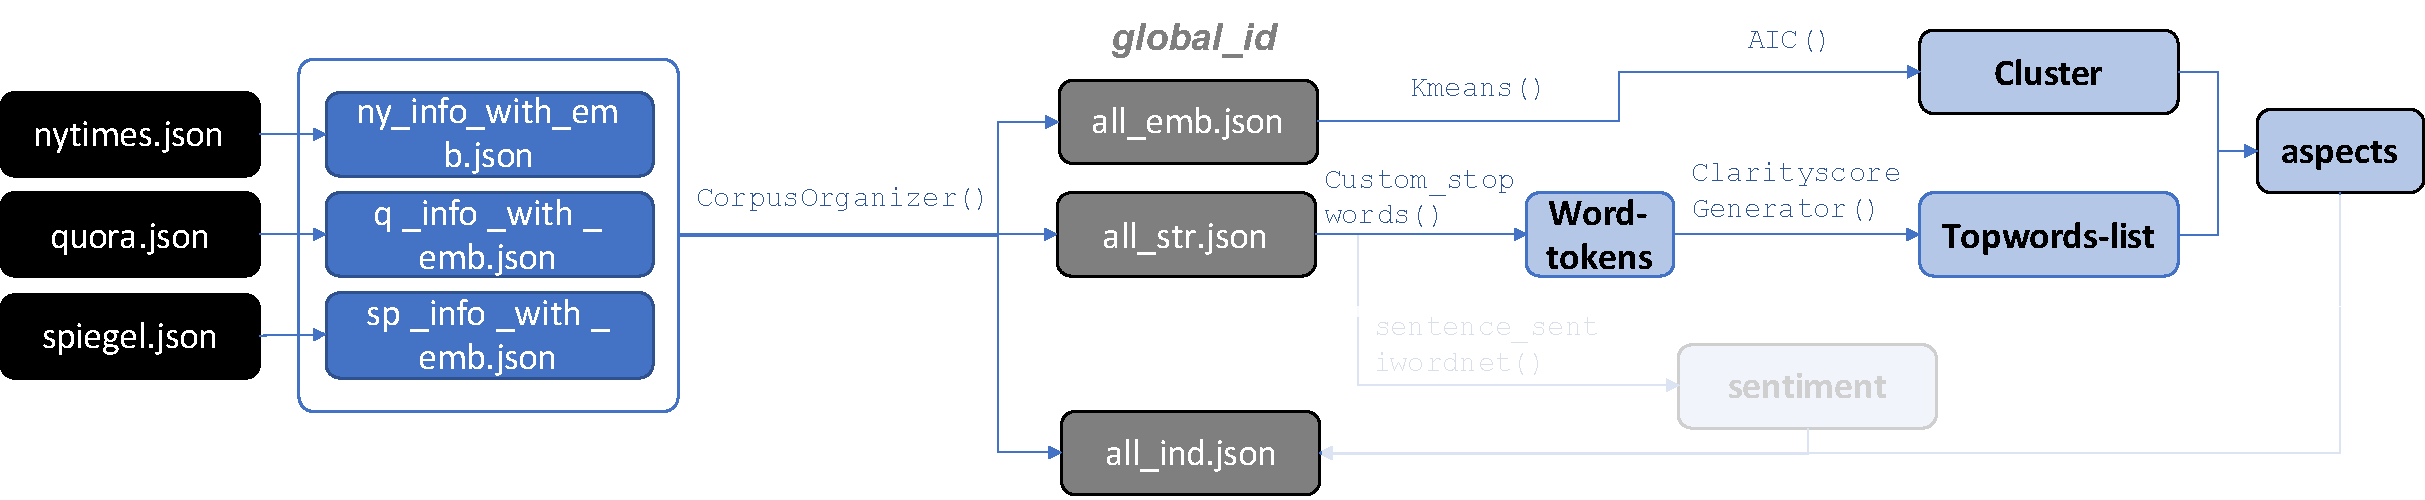
\includegraphics[width = \textwidth]{figures/journey1.pdf}
    \end{figure}

Example sentence: \textit{"Like most grocery chains, Whole Foods does not release sales data on individual stores."}
\\[2ex]
\begin{tabular}{|r|l|r|r|r|}
      global\_id & corpus\_name &  doc\_id &  com\_id  &  \textbf{cluster} \\
     
      30120 &     nytimes &     191 &     NaN &        \textbf{7} \\
      \end{tabular}
\end{frame}

\begin{frame}
  \frametitle{Sentiment Analysis}
  \framesubtitle{first try: Vader Sentiment \footcite{hutto2014vader}}
  \begin{description}
    \large
    \item Features
    \item \begin{itemize}
      \item  working directly on sentence-level 
      \item  pre-trained on social media like tweets, nytimes, movie reviews courpus 
    \end{itemize}
    \vspace{0.2cm}
    \item Drawbacks
    \item \begin{itemize}
      \item  No multilingual
      \item  only work for simple comments on social media, limited by their pre-training corpus
    \end{itemize}
    \vspace{0.2cm}
    \item Example
    \item "... McDonald's will soon be serving a coffee that comes from organic beans and is certified ..." 
    \item result: \{'compound': 0.3182, 'neg': 0.0, 'neu': 0.943, 'pos': 0.057\}
  \end{description}
\end{frame}

\begin{frame}
  \frametitle{Sentiment Analysis}
  \framesubtitle{second try: Sentiwordnet \footcite{minemyopinion} \&  SentiWS\footcite{remus2010sentiws}}     
  \begin{description}
    \large
    \item Features
    \item \begin{itemize}
      \item  based on POS (part-of-speech) tagging: ADJ,NOUN,ADV,VERB
      \item  EN: using synset (synonym set) to compute average sentiment score
      \item  DE: semantic orientation based on PMI \footcite{remus2010sentiws}    
      \item  sentiment strength score:  $\in [-1,1]$ 
    \end{itemize}
    \vspace{0.2cm}
    \item Example:
    \item "Like most grocery chains, Whole Foods does not release sales data on individual stores." 
    \item ('Like', 'IN'), ('most', 'JJS'), ('grocery', 'NN'), ('chains', 'NNS'), (',', ','), ('Whole', 'NNP'),...
    \item result: -0.625
  \end{description}
\end{frame}

\begin{frame}
  \frametitle{Back to our journey}
    
  \begin{figure}[t]
    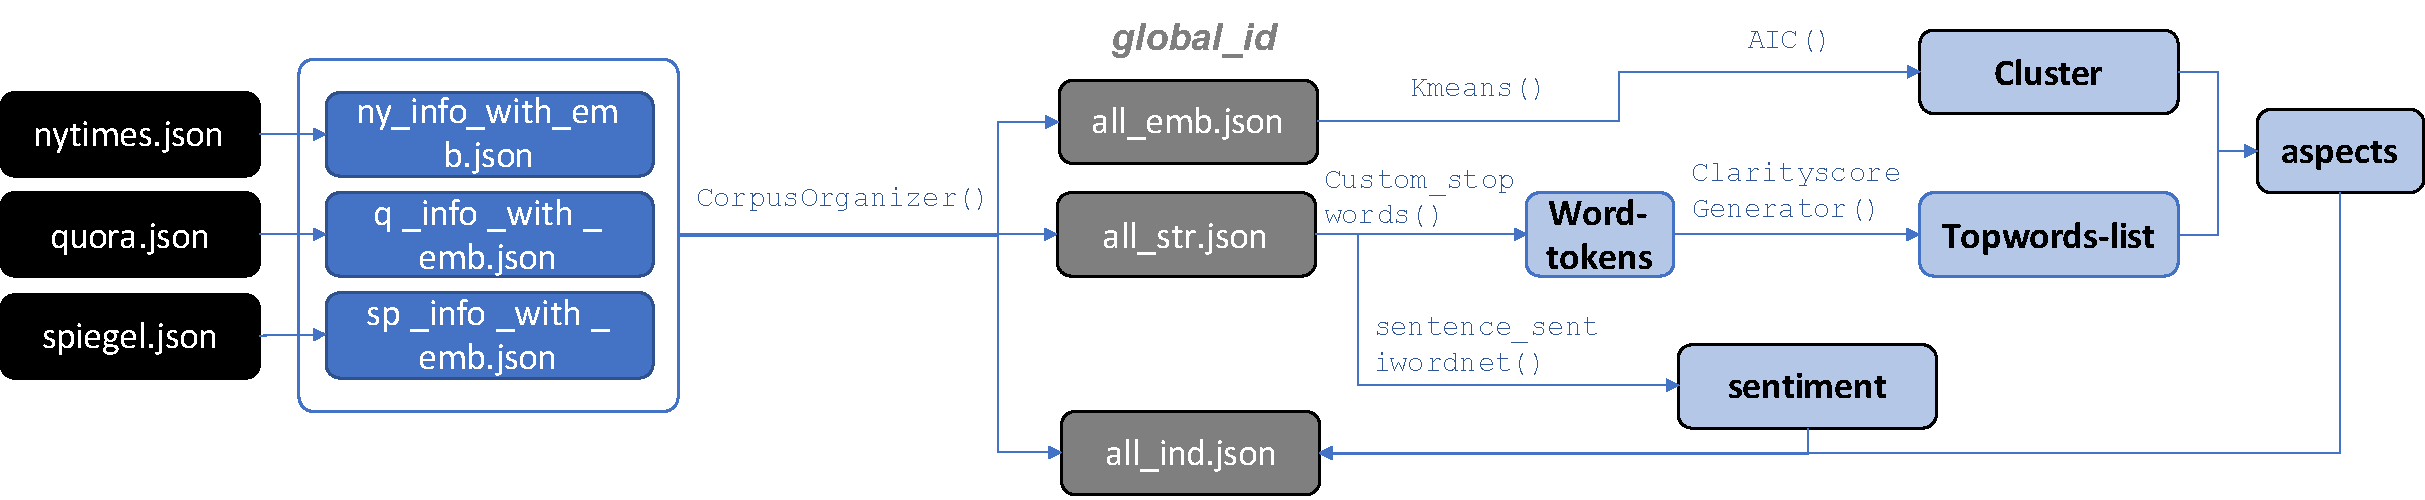
\includegraphics[width = \textwidth]{figures/journey.pdf}
    \end{figure}

    Example sentence: \textit{"Like most grocery chains, Whole Foods does not release sales data on individual stores."}
\\[2ex]
  \begin{tabular}{|r|l|r|r|r|r|}
    global\_id & corpus\_name &  doc\_id &  com\_id &  \textbf{cluster} &  \textbf{sentiment} \\
   
    30120 &     nytimes &     191 &     NaN &        \textbf{7} &     \textbf{-0.625} \\
    \end{tabular}

    
\end{frame}


\section{Stage 2: Distribution}
\begin{frame}[fragile]
  \frametitle{Accumulating and Normalizing (naive approach)}
  \begin{description}
    \large

    \item accumulate all sentences tuple \textbf{(<cluster>,<sentiment>)}
    \begin{lstlisting}
      cluster_group = doc.groupby('cluster')
      for (_,cluster) in cluster_group:
        label = cluster.cluster.unique()[0]
        doc_dic[label] = sum([abs(x) for x in scores]), sum([x for x in scores if x>0])
      \end{lstlisting}
      \item normalize
    
      \begin{lstlisting}
        df_new_t['normalized_pos'] = (df_new_t[1])/all_abs_sum
        df_new_t['normalized_neg'] = (df_new_t[2])/all_abs_sum
  
    \end{lstlisting}
    \item Example:
    \small
    \begin{tabular}{lrr}
    
      {} &  normalized\_pos &  normalized\_neg \\
     
      Chemicals \& Cancer &        0.000000 &       -0.023515 \\
      Meat \& Animals     &        0.032921 &       -0.028218 \\
      Health \& Diet      &        0.000000 &       -0.009406 \\
      Retail             &        0.206930 &       -0.069604 \\
      GMO                &        0.157471 &       -0.289232 \\
      Agriculture        &        0.058858 &       -0.089356 \\
      Polices            &        0.031353 &        0.000000 \\
      Economy            &        0.003135 &        0.000000 \\
      
      \end{tabular}
  \end{description}
\end{frame}


\subsection{2.1 Representing one article}
\begin{frame}
  \frametitle{Representing NYTimes articles}
  \begin{columns}[t]
    \column{.5\textwidth}
    \centering
    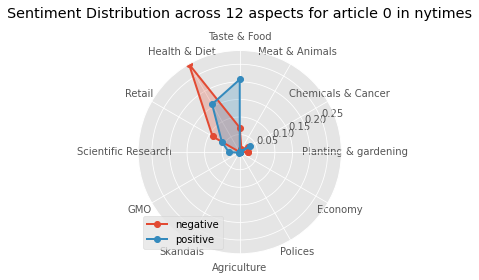
\includegraphics[width = \textwidth]{figures/radar_nytimes_0.png}\\
    \column{.5\textwidth}
    \centering
    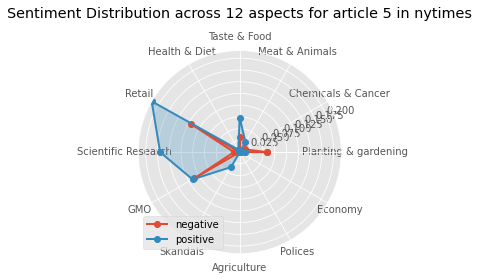
\includegraphics[width = \textwidth]{figures/radar_nytimes_5.png}
    \end{columns}
    
\end{frame}

\begin{frame}
  \frametitle{Representing Spiegel articles}
  \begin{columns}[t]
    \column{.5\textwidth}
    \centering
    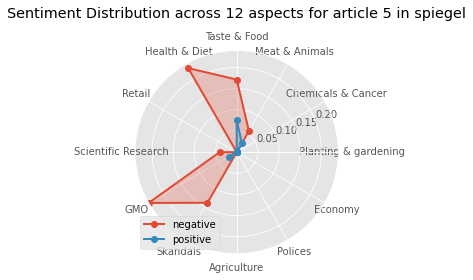
\includegraphics[width = \textwidth]{figures/radar_spiegel_5.png}\\
    \column{.5\textwidth}
    \centering
    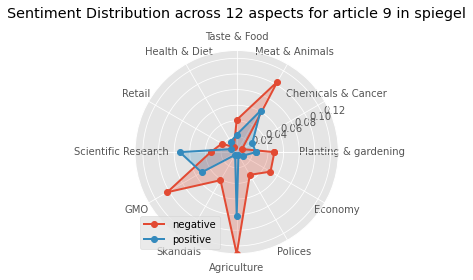
\includegraphics[width = \textwidth]{figures/radar_spiegel_9.png}
    \end{columns}
    
\end{frame}


\subsection{2.2 Distribution on whole corpus}
\begin{frame}
  \frametitle{Distribution on whole corpus (without comments)}
  In total there are 875 documents.
  nytimes has 327 documents.
  quora has 396 documents. (there are more articles that only have comments)
  spiegel has 152 documents.
\\[2ex]
\begin{minipage}{0.5\linewidth}
    \begin{center}
    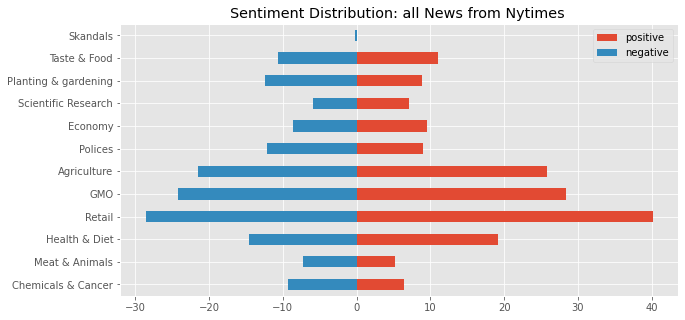
\includegraphics[width = 1\textwidth]{figures/nytimes_sentiments_2.png}
    \captionof{figure}{All articles from NYTimes}
    \end{center}
  \end{minipage}%
  \hfill
    \begin{minipage}{0.5\linewidth}
    \begin{center}
    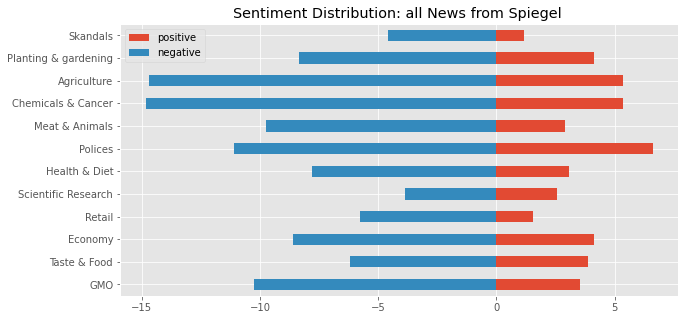
\includegraphics[width = 1\textwidth]{figures/spiegel_sentiments_2.png}
    \captionof{figure}{All articles from Spiegel}
    \end{center}
  \end{minipage}%
  \hfill

    %\includegraphics[width = 0.45\textwidth]{figures/quora_sentiments.png}
\end{frame}


\subsection{2.3 Calculation of CF-IDF}
\begin{frame}
  \frametitle{Concept frequency - inverse document frequency (CF-IDF)}
  \begin{center}
    \begin{figure}[t]
      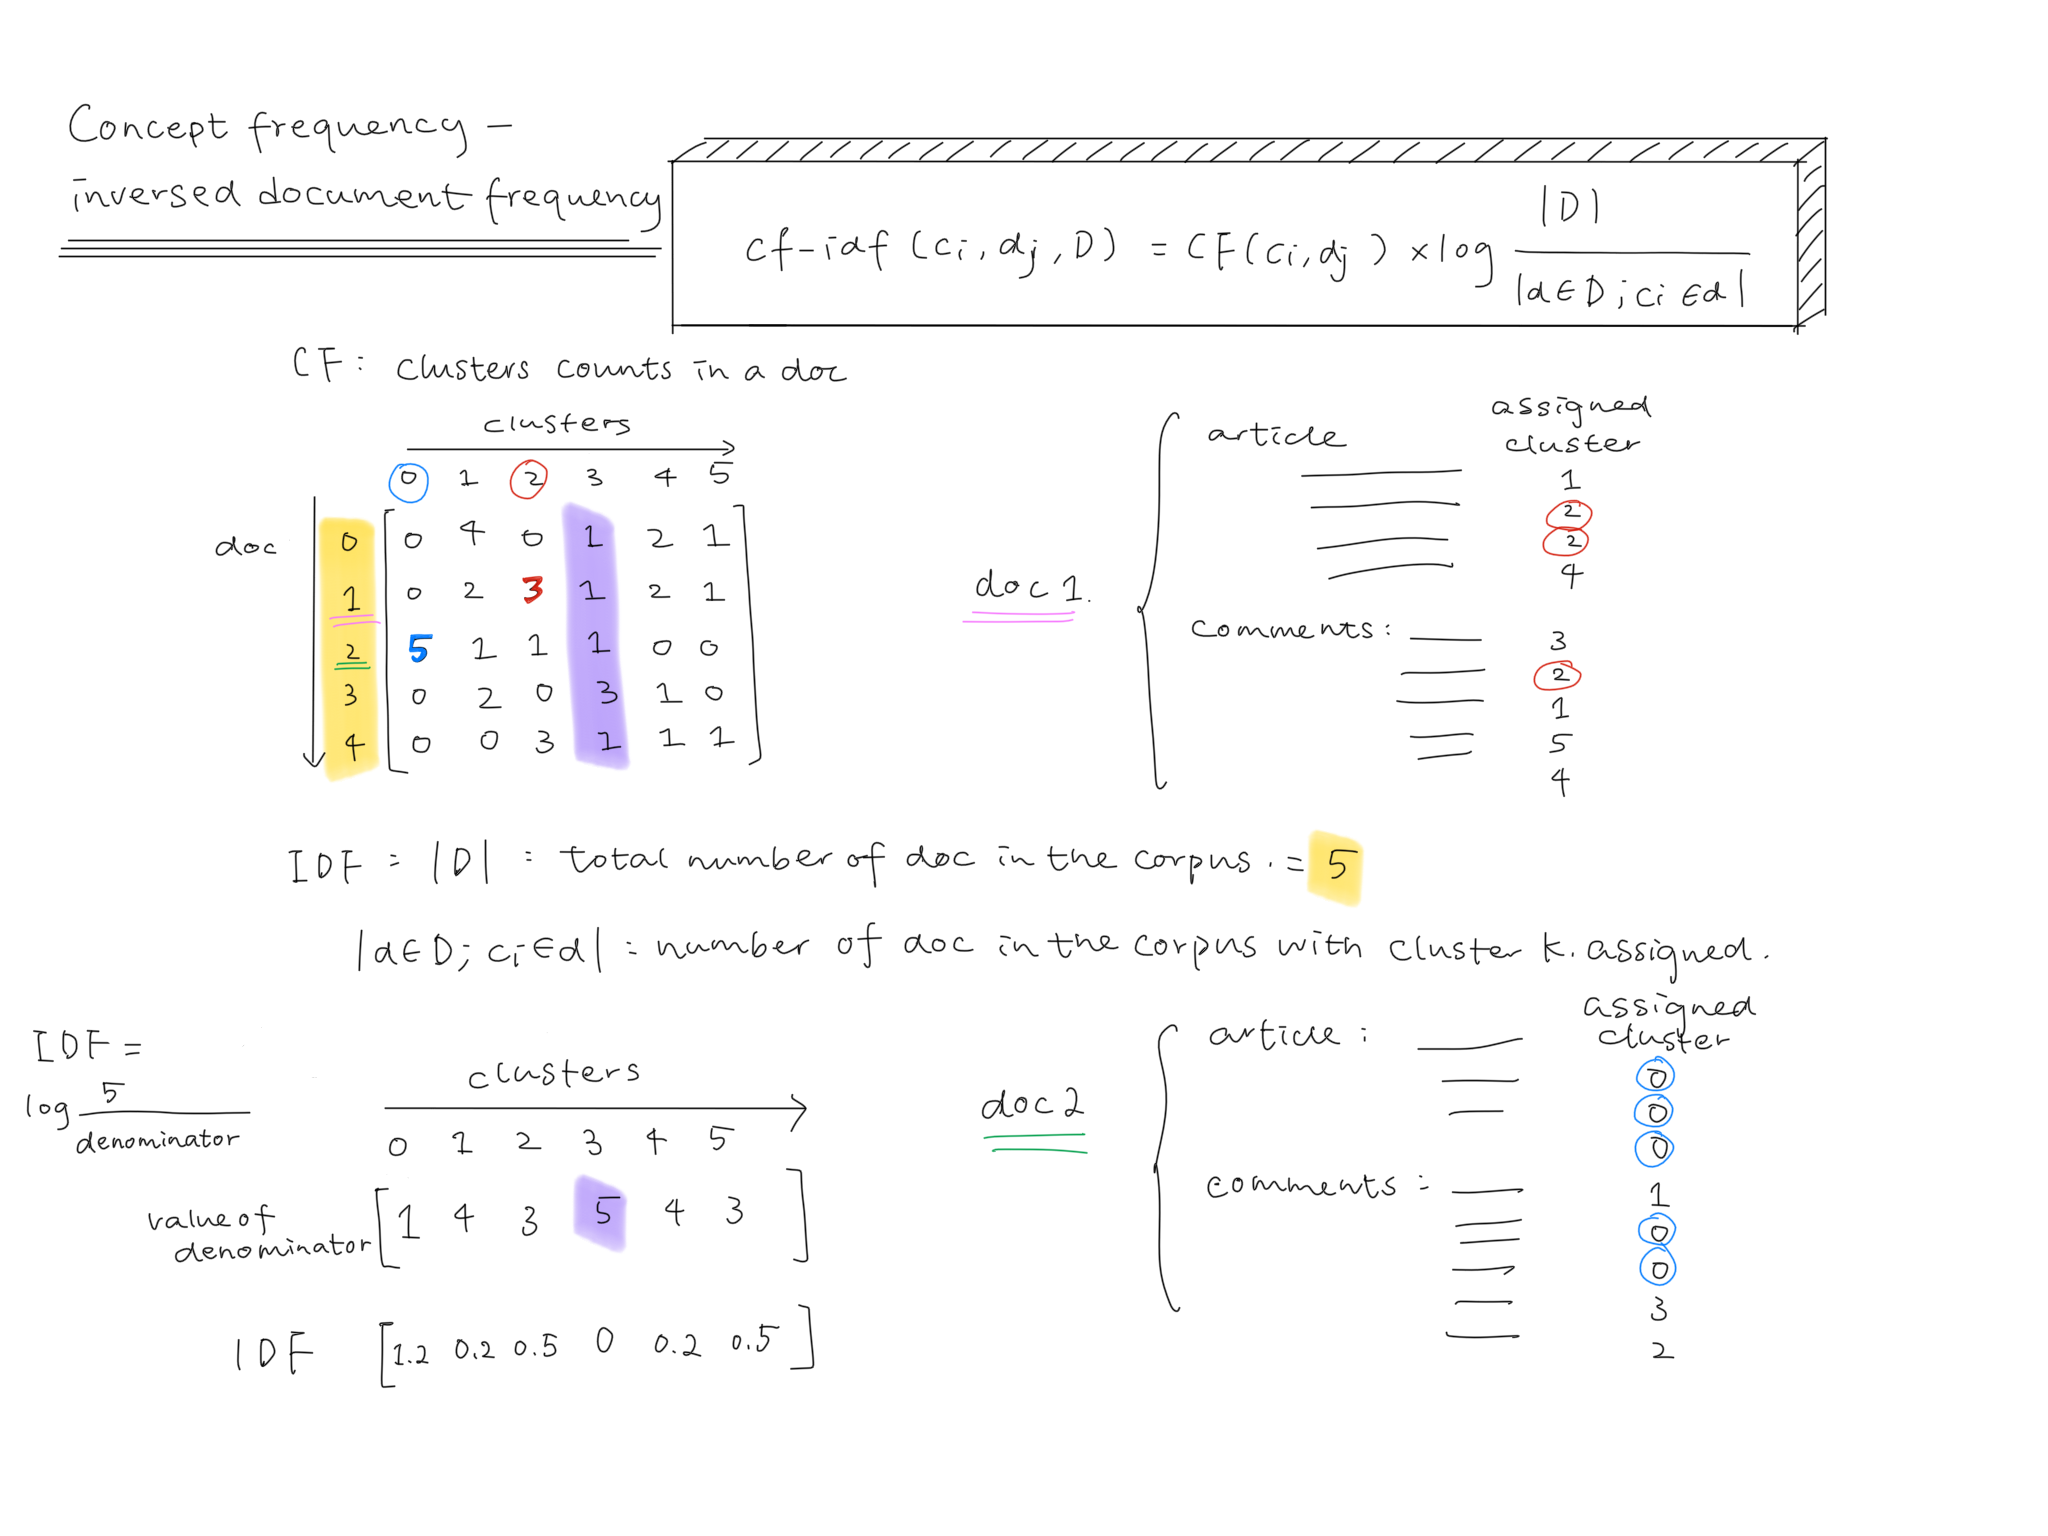
\includegraphics[width=0.6\textwidth]{images/CF-IDF_concept.png}
    \end{figure}
  \end{center}
\end{frame}

\begin{frame}[fragile]
  \frametitle{CF-IDF results}
  \begin{lstlisting}
IDF = np.log(TOTAL_NUM_OF_DOC / num_of_doc_per_cluster)
CFIDF = CF * IDF
print(CF[0:3], IDF, CFIDF[0:3])
  \end{lstlisting}
  \begin{center}
    \begin{figure}[t]
      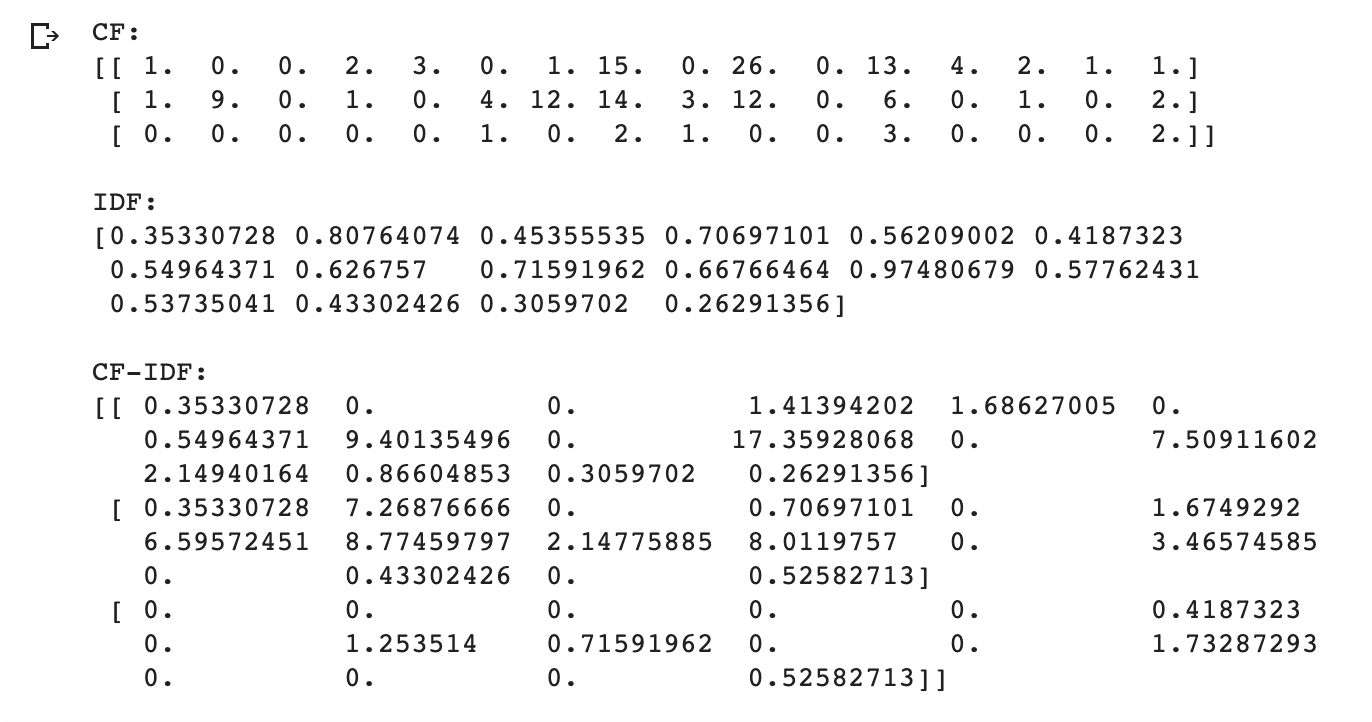
\includegraphics[width=0.6\textwidth]{images/CF-IDF_result.png}
      \caption{Sample output for first 3 documents and IDF for the whole corpus}
    \end{figure}
  \end{center}
\end{frame}

\begin{frame}
 \frametitle{CF-IDF radar plot example}
 \subframetitle{}
 \begin{center}
    \begin{figure}[t]
      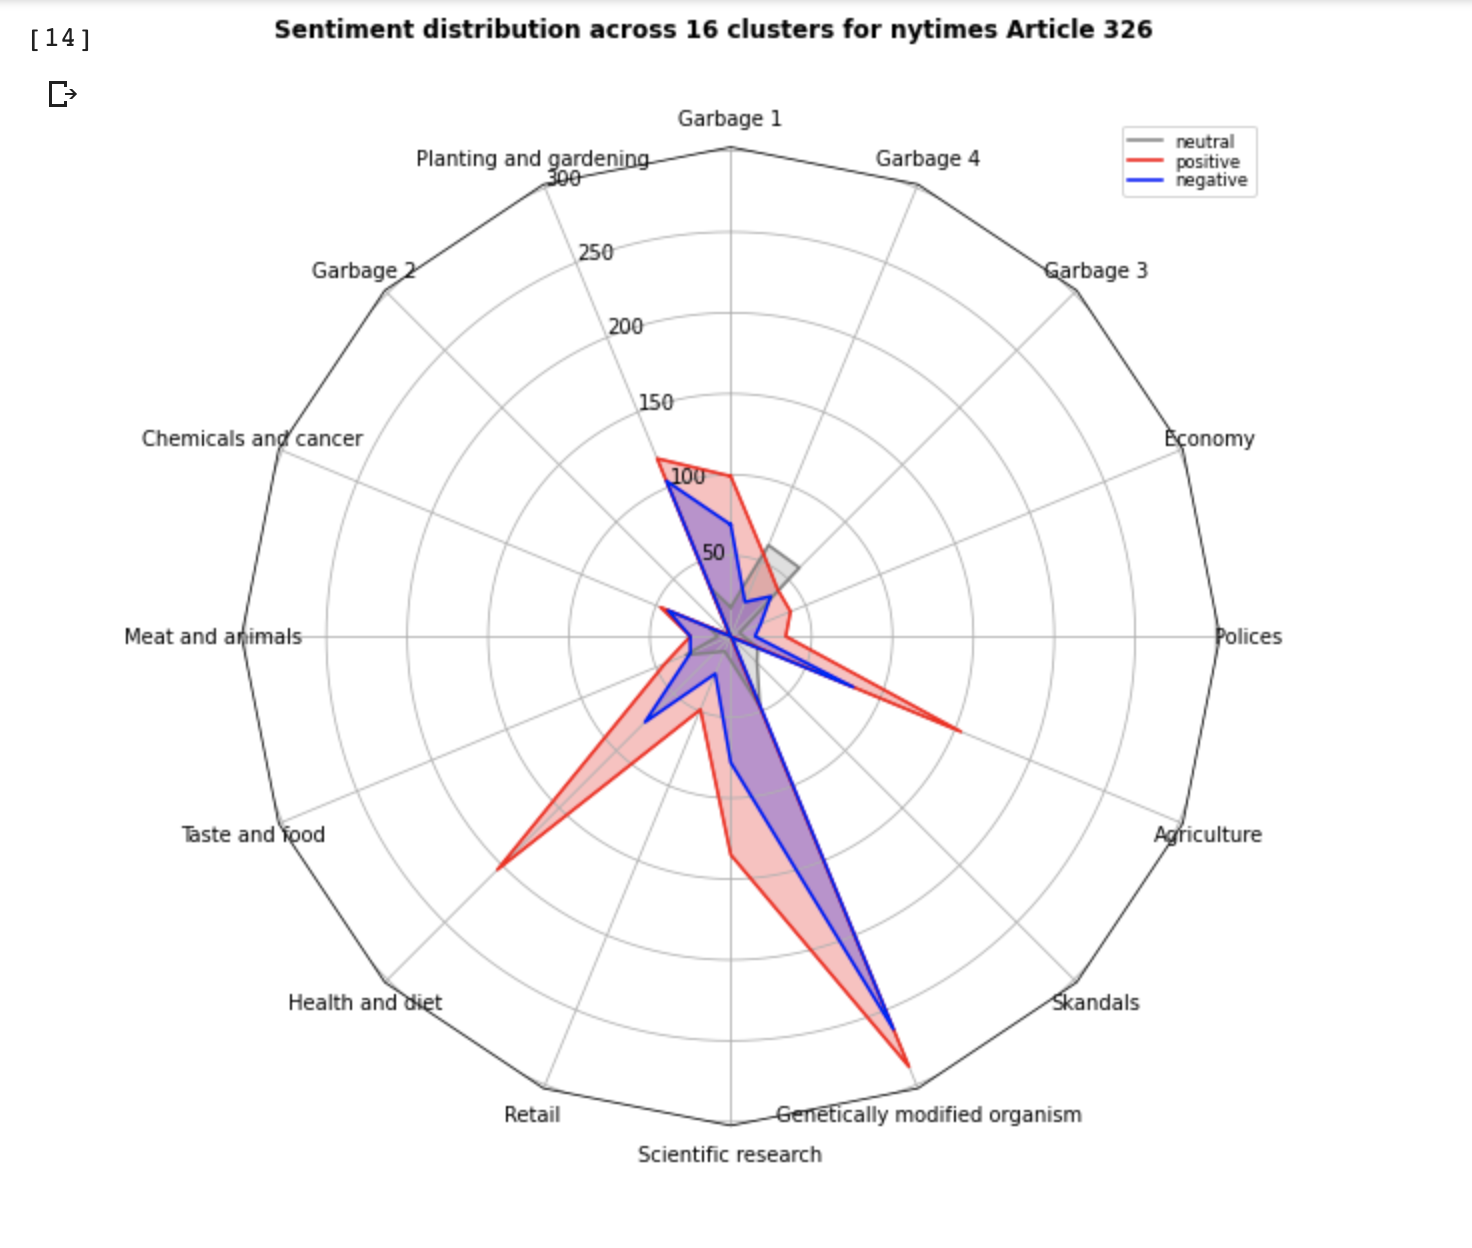
\includegraphics[width=0.4\textwidth]{images/CF-IDF-nytimes-326.png}
      \caption{$\text{value} = \text{CF-IDF} \times \text{number of sentiments}$}
    \end{figure}
  \end{center}   
\end{frame}


\section{Future Plan}
\begin{frame}
  \frametitle{Next Plan}
  \large
  \begin{itemize}
    \item  To represent the newspaper article and its comments (separately?) using CF-IDF
    \item  To analysis the correlations between articles of NYTimes and comments of NYTimes
  \end{itemize}
\end{frame}
\begin{frame}
  \frametitle{References}
 
  \printbibliography

\end{frame}
\end{document}